% Created by tikzDevice version 0.10.1 on 2020-02-15 16:04:44
% !TEX encoding = UTF-8 Unicode
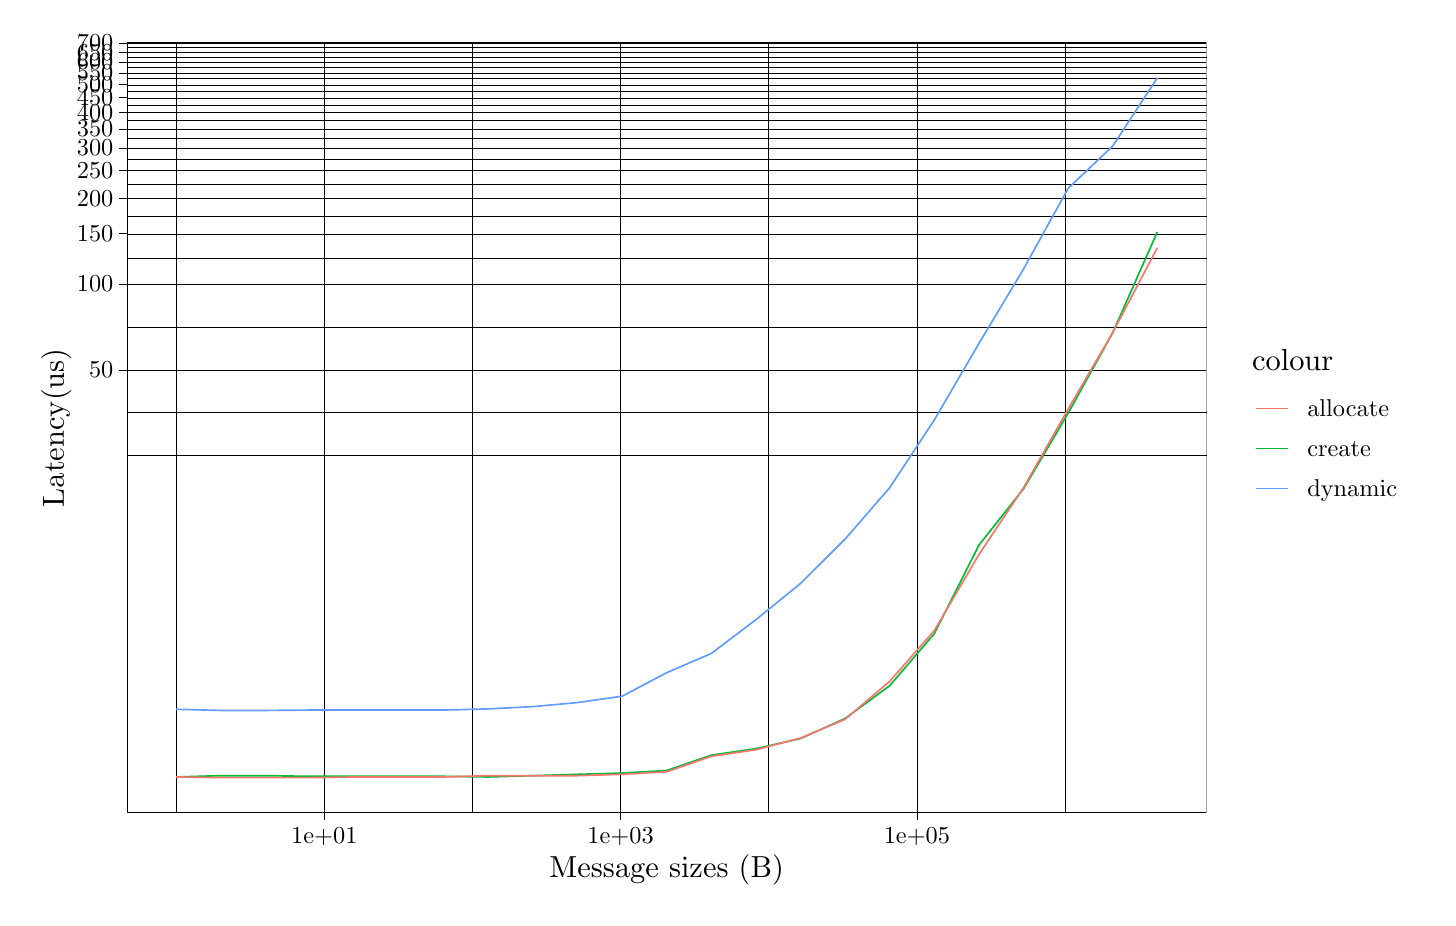
\begin{tikzpicture}[x=1pt,y=1pt]
\definecolor{fillColor}{RGB}{255,255,255}
\path[use as bounding box,fill=fillColor,fill opacity=0.00] (0,0) rectangle (505.89,314.37);
\begin{scope}
\path[clip] (  0.00,  0.00) rectangle (505.89,314.37);
\definecolor{drawColor}{RGB}{255,255,255}
\definecolor{fillColor}{RGB}{255,255,255}

\path[draw=drawColor,line width= 0.6pt,line join=round,line cap=round,fill=fillColor] (  0.00,  0.00) rectangle (505.89,314.37);
\end{scope}
\begin{scope}
\path[clip] ( 35.92, 30.72) rectangle (425.93,308.87);
\definecolor{fillColor}{RGB}{255,255,255}

\path[fill=fillColor] ( 35.92, 30.72) rectangle (425.93,308.87);
\definecolor{drawColor}{RGB}{0,0,0}

\path[draw=drawColor,line width= 0.0pt,line join=round] ( 35.92,159.66) --
	(425.93,159.66);

\path[draw=drawColor,line width= 0.0pt,line join=round] ( 35.92,175.17) --
	(425.93,175.17);

\path[draw=drawColor,line width= 0.0pt,line join=round] ( 35.92,206.20) --
	(425.93,206.20);

\path[draw=drawColor,line width= 0.0pt,line join=round] ( 35.92,230.78) --
	(425.93,230.78);

\path[draw=drawColor,line width= 0.0pt,line join=round] ( 35.92,246.29) --
	(425.93,246.29);

\path[draw=drawColor,line width= 0.0pt,line join=round] ( 35.92,257.72) --
	(425.93,257.72);

\path[draw=drawColor,line width= 0.0pt,line join=round] ( 35.92,266.80) --
	(425.93,266.80);

\path[draw=drawColor,line width= 0.0pt,line join=round] ( 35.92,274.33) --
	(425.93,274.33);

\path[draw=drawColor,line width= 0.0pt,line join=round] ( 35.92,280.77) --
	(425.93,280.77);

\path[draw=drawColor,line width= 0.0pt,line join=round] ( 35.92,286.39) --
	(425.93,286.39);

\path[draw=drawColor,line width= 0.0pt,line join=round] ( 35.92,291.38) --
	(425.93,291.38);

\path[draw=drawColor,line width= 0.0pt,line join=round] ( 35.92,295.87) --
	(425.93,295.87);

\path[draw=drawColor,line width= 0.0pt,line join=round] ( 35.92,299.95) --
	(425.93,299.95);

\path[draw=drawColor,line width= 0.0pt,line join=round] ( 35.92,303.69) --
	(425.93,303.69);

\path[draw=drawColor,line width= 0.0pt,line join=round] ( 35.92,307.14) --
	(425.93,307.14);

\path[draw=drawColor,line width= 0.0pt,line join=round] ( 53.64, 30.72) --
	( 53.64,308.87);

\path[draw=drawColor,line width= 0.0pt,line join=round] (160.72, 30.72) --
	(160.72,308.87);

\path[draw=drawColor,line width= 0.0pt,line join=round] (267.79, 30.72) --
	(267.79,308.87);

\path[draw=drawColor,line width= 0.0pt,line join=round] (374.87, 30.72) --
	(374.87,308.87);

\path[draw=drawColor,line width= 0.1pt,line join=round] ( 35.92,190.68) --
	(425.93,190.68);

\path[draw=drawColor,line width= 0.1pt,line join=round] ( 35.92,221.71) --
	(425.93,221.71);

\path[draw=drawColor,line width= 0.1pt,line join=round] ( 35.92,239.85) --
	(425.93,239.85);

\path[draw=drawColor,line width= 0.1pt,line join=round] ( 35.92,252.73) --
	(425.93,252.73);

\path[draw=drawColor,line width= 0.1pt,line join=round] ( 35.92,262.72) --
	(425.93,262.72);

\path[draw=drawColor,line width= 0.1pt,line join=round] ( 35.92,270.88) --
	(425.93,270.88);

\path[draw=drawColor,line width= 0.1pt,line join=round] ( 35.92,277.78) --
	(425.93,277.78);

\path[draw=drawColor,line width= 0.1pt,line join=round] ( 35.92,283.75) --
	(425.93,283.75);

\path[draw=drawColor,line width= 0.1pt,line join=round] ( 35.92,289.03) --
	(425.93,289.03);

\path[draw=drawColor,line width= 0.1pt,line join=round] ( 35.92,293.74) --
	(425.93,293.74);

\path[draw=drawColor,line width= 0.1pt,line join=round] ( 35.92,298.01) --
	(425.93,298.01);

\path[draw=drawColor,line width= 0.1pt,line join=round] ( 35.92,301.90) --
	(425.93,301.90);

\path[draw=drawColor,line width= 0.1pt,line join=round] ( 35.92,305.48) --
	(425.93,305.48);

\path[draw=drawColor,line width= 0.1pt,line join=round] ( 35.92,308.80) --
	(425.93,308.80);

\path[draw=drawColor,line width= 0.1pt,line join=round] (107.18, 30.72) --
	(107.18,308.87);

\path[draw=drawColor,line width= 0.1pt,line join=round] (214.26, 30.72) --
	(214.26,308.87);

\path[draw=drawColor,line width= 0.1pt,line join=round] (321.33, 30.72) --
	(321.33,308.87);
\definecolor{drawColor}{RGB}{0,186,56}

\path[draw=drawColor,line width= 0.6pt,line join=round] ( 53.64, 43.61) --
	( 69.76, 44.08) --
	( 85.88, 44.08) --
	(101.99, 43.85) --
	(118.11, 43.85) --
	(134.23, 43.85) --
	(150.34, 43.85) --
	(166.46, 43.61) --
	(182.58, 44.08) --
	(198.69, 44.56) --
	(214.81, 45.02) --
	(230.92, 45.94) --
	(247.04, 51.49) --
	(263.16, 53.83) --
	(279.27, 57.49) --
	(295.39, 64.76) --
	(311.51, 76.62) --
	(327.62, 95.41) --
	(343.74,127.40) --
	(359.86,147.75) --
	(375.97,175.08) --
	(392.09,204.17) --
	(408.20,240.59);
\definecolor{drawColor}{RGB}{248,118,109}

\path[draw=drawColor,line width= 0.6pt,line join=round] ( 53.64, 43.61) --
	( 69.76, 43.37) --
	( 85.88, 43.37) --
	(101.99, 43.37) --
	(118.11, 43.61) --
	(134.23, 43.61) --
	(150.34, 43.61) --
	(166.46, 44.08) --
	(182.58, 44.08) --
	(198.69, 44.08) --
	(214.81, 44.56) --
	(230.92, 45.48) --
	(247.04, 51.08) --
	(263.16, 53.45) --
	(279.27, 57.66) --
	(295.39, 64.46) --
	(311.51, 78.20) --
	(327.62, 96.53) --
	(343.74,124.00) --
	(359.86,148.17) --
	(375.97,176.55) --
	(392.09,204.24) --
	(408.20,234.84);
\definecolor{drawColor}{RGB}{97,156,255}

\path[draw=drawColor,line width= 0.6pt,line join=round] ( 53.64, 68.07) --
	( 69.76, 67.65) --
	( 85.88, 67.65) --
	(101.99, 67.79) --
	(118.11, 67.79) --
	(134.23, 67.79) --
	(150.34, 67.79) --
	(166.46, 68.21) --
	(182.58, 69.03) --
	(198.69, 70.50) --
	(214.81, 72.80) --
	(230.92, 81.29) --
	(247.04, 88.25) --
	(263.16,100.46) --
	(279.27,113.53) --
	(295.39,129.59) --
	(311.51,148.17) --
	(327.62,172.64) --
	(343.74,200.28) --
	(359.86,227.17) --
	(375.97,256.30) --
	(392.09,271.61) --
	(408.20,296.23);
\definecolor{drawColor}{RGB}{0,0,0}

\path[draw=drawColor,line width= 0.6pt,line join=round,line cap=round] ( 35.92, 30.72) rectangle (425.93,308.87);
\end{scope}
\begin{scope}
\path[clip] (  0.00,  0.00) rectangle (505.89,314.37);
\definecolor{drawColor}{RGB}{0,0,0}

\node[text=drawColor,anchor=base west,inner sep=0pt, outer sep=0pt, scale=  0.88] at ( 22.17,187.86) {50};

\node[text=drawColor,anchor=base west,inner sep=0pt, outer sep=0pt, scale=  0.88] at ( 17.77,218.88) {100};

\node[text=drawColor,anchor=base west,inner sep=0pt, outer sep=0pt, scale=  0.88] at ( 17.77,237.03) {150};

\node[text=drawColor,anchor=base west,inner sep=0pt, outer sep=0pt, scale=  0.88] at ( 17.77,249.91) {200};

\node[text=drawColor,anchor=base west,inner sep=0pt, outer sep=0pt, scale=  0.88] at ( 17.77,259.89) {250};

\node[text=drawColor,anchor=base west,inner sep=0pt, outer sep=0pt, scale=  0.88] at ( 17.77,268.06) {300};

\node[text=drawColor,anchor=base west,inner sep=0pt, outer sep=0pt, scale=  0.88] at ( 17.77,274.95) {350};

\node[text=drawColor,anchor=base west,inner sep=0pt, outer sep=0pt, scale=  0.88] at ( 17.77,280.93) {400};

\node[text=drawColor,anchor=base west,inner sep=0pt, outer sep=0pt, scale=  0.88] at ( 17.77,286.20) {450};

\node[text=drawColor,anchor=base west,inner sep=0pt, outer sep=0pt, scale=  0.88] at ( 17.77,290.92) {500};

\node[text=drawColor,anchor=base west,inner sep=0pt, outer sep=0pt, scale=  0.88] at ( 17.77,295.18) {550};

\node[text=drawColor,anchor=base west,inner sep=0pt, outer sep=0pt, scale=  0.88] at ( 17.77,299.08) {600};

\node[text=drawColor,anchor=base west,inner sep=0pt, outer sep=0pt, scale=  0.88] at ( 17.77,302.66) {650};

\node[text=drawColor,anchor=base west,inner sep=0pt, outer sep=0pt, scale=  0.88] at ( 17.77,305.98) {700};
\end{scope}
\begin{scope}
\path[clip] (  0.00,  0.00) rectangle (505.89,314.37);
\definecolor{drawColor}{RGB}{0,0,0}

\path[draw=drawColor,line width= 0.3pt,line join=round] ( 33.17,190.68) --
	( 35.92,190.68);

\path[draw=drawColor,line width= 0.3pt,line join=round] ( 33.17,221.71) --
	( 35.92,221.71);

\path[draw=drawColor,line width= 0.3pt,line join=round] ( 33.17,239.85) --
	( 35.92,239.85);

\path[draw=drawColor,line width= 0.3pt,line join=round] ( 33.17,252.73) --
	( 35.92,252.73);

\path[draw=drawColor,line width= 0.3pt,line join=round] ( 33.17,262.72) --
	( 35.92,262.72);

\path[draw=drawColor,line width= 0.3pt,line join=round] ( 33.17,270.88) --
	( 35.92,270.88);

\path[draw=drawColor,line width= 0.3pt,line join=round] ( 33.17,277.78) --
	( 35.92,277.78);

\path[draw=drawColor,line width= 0.3pt,line join=round] ( 33.17,283.75) --
	( 35.92,283.75);

\path[draw=drawColor,line width= 0.3pt,line join=round] ( 33.17,289.03) --
	( 35.92,289.03);

\path[draw=drawColor,line width= 0.3pt,line join=round] ( 33.17,293.74) --
	( 35.92,293.74);

\path[draw=drawColor,line width= 0.3pt,line join=round] ( 33.17,298.01) --
	( 35.92,298.01);

\path[draw=drawColor,line width= 0.3pt,line join=round] ( 33.17,301.90) --
	( 35.92,301.90);

\path[draw=drawColor,line width= 0.3pt,line join=round] ( 33.17,305.48) --
	( 35.92,305.48);

\path[draw=drawColor,line width= 0.3pt,line join=round] ( 33.17,308.80) --
	( 35.92,308.80);
\end{scope}
\begin{scope}
\path[clip] (  0.00,  0.00) rectangle (505.89,314.37);
\definecolor{drawColor}{RGB}{0,0,0}

\path[draw=drawColor,line width= 0.3pt,line join=round] (107.18, 27.97) --
	(107.18, 30.72);

\path[draw=drawColor,line width= 0.3pt,line join=round] (214.26, 27.97) --
	(214.26, 30.72);

\path[draw=drawColor,line width= 0.3pt,line join=round] (321.33, 27.97) --
	(321.33, 30.72);
\end{scope}
\begin{scope}
\path[clip] (  0.00,  0.00) rectangle (505.89,314.37);
\definecolor{drawColor}{RGB}{0,0,0}

\node[text=drawColor,anchor=base,inner sep=0pt, outer sep=0pt, scale=  0.88] at (107.18, 19.71) {1e+01};

\node[text=drawColor,anchor=base,inner sep=0pt, outer sep=0pt, scale=  0.88] at (214.26, 19.71) {1e+03};

\node[text=drawColor,anchor=base,inner sep=0pt, outer sep=0pt, scale=  0.88] at (321.33, 19.71) {1e+05};
\end{scope}
\begin{scope}
\path[clip] (  0.00,  0.00) rectangle (505.89,314.37);
\definecolor{drawColor}{RGB}{0,0,0}

\node[text=drawColor,anchor=base,inner sep=0pt, outer sep=0pt, scale=  1.10] at (230.92,  7.44) {Message sizes (B)};
\end{scope}
\begin{scope}
\path[clip] (  0.00,  0.00) rectangle (505.89,314.37);
\definecolor{drawColor}{RGB}{0,0,0}

\node[text=drawColor,rotate= 90.00,anchor=base,inner sep=0pt, outer sep=0pt, scale=  1.10] at ( 13.08,169.80) {Latency(us)};
\end{scope}
\begin{scope}
\path[clip] (  0.00,  0.00) rectangle (505.89,314.37);
\definecolor{fillColor}{RGB}{255,255,255}

\path[fill=fillColor] (436.93,135.11) rectangle (500.39,204.49);
\end{scope}
\begin{scope}
\path[clip] (  0.00,  0.00) rectangle (505.89,314.37);
\definecolor{drawColor}{RGB}{0,0,0}

\node[text=drawColor,anchor=base west,inner sep=0pt, outer sep=0pt, scale=  1.10] at (442.43,190.44) {colour};
\end{scope}
\begin{scope}
\path[clip] (  0.00,  0.00) rectangle (505.89,314.37);
\definecolor{fillColor}{RGB}{255,255,255}

\path[fill=fillColor] (442.43,169.52) rectangle (456.89,183.97);
\end{scope}
\begin{scope}
\path[clip] (  0.00,  0.00) rectangle (505.89,314.37);
\definecolor{drawColor}{RGB}{248,118,109}

\path[draw=drawColor,line width= 0.6pt,line join=round] (443.88,176.74) -- (455.44,176.74);
\end{scope}
\begin{scope}
\path[clip] (  0.00,  0.00) rectangle (505.89,314.37);
\definecolor{drawColor}{RGB}{248,118,109}

\path[draw=drawColor,line width= 0.6pt,line join=round] (443.88,176.74) -- (455.44,176.74);
\end{scope}
\begin{scope}
\path[clip] (  0.00,  0.00) rectangle (505.89,314.37);
\definecolor{drawColor}{RGB}{248,118,109}

\path[draw=drawColor,line width= 0.6pt,line join=round] (443.88,176.74) -- (455.44,176.74);
\end{scope}
\begin{scope}
\path[clip] (  0.00,  0.00) rectangle (505.89,314.37);
\definecolor{fillColor}{RGB}{255,255,255}

\path[fill=fillColor] (442.43,155.06) rectangle (456.89,169.52);
\end{scope}
\begin{scope}
\path[clip] (  0.00,  0.00) rectangle (505.89,314.37);
\definecolor{drawColor}{RGB}{0,186,56}

\path[draw=drawColor,line width= 0.6pt,line join=round] (443.88,162.29) -- (455.44,162.29);
\end{scope}
\begin{scope}
\path[clip] (  0.00,  0.00) rectangle (505.89,314.37);
\definecolor{drawColor}{RGB}{0,186,56}

\path[draw=drawColor,line width= 0.6pt,line join=round] (443.88,162.29) -- (455.44,162.29);
\end{scope}
\begin{scope}
\path[clip] (  0.00,  0.00) rectangle (505.89,314.37);
\definecolor{drawColor}{RGB}{0,186,56}

\path[draw=drawColor,line width= 0.6pt,line join=round] (443.88,162.29) -- (455.44,162.29);
\end{scope}
\begin{scope}
\path[clip] (  0.00,  0.00) rectangle (505.89,314.37);
\definecolor{fillColor}{RGB}{255,255,255}

\path[fill=fillColor] (442.43,140.61) rectangle (456.89,155.06);
\end{scope}
\begin{scope}
\path[clip] (  0.00,  0.00) rectangle (505.89,314.37);
\definecolor{drawColor}{RGB}{97,156,255}

\path[draw=drawColor,line width= 0.6pt,line join=round] (443.88,147.84) -- (455.44,147.84);
\end{scope}
\begin{scope}
\path[clip] (  0.00,  0.00) rectangle (505.89,314.37);
\definecolor{drawColor}{RGB}{97,156,255}

\path[draw=drawColor,line width= 0.6pt,line join=round] (443.88,147.84) -- (455.44,147.84);
\end{scope}
\begin{scope}
\path[clip] (  0.00,  0.00) rectangle (505.89,314.37);
\definecolor{drawColor}{RGB}{97,156,255}

\path[draw=drawColor,line width= 0.6pt,line join=round] (443.88,147.84) -- (455.44,147.84);
\end{scope}
\begin{scope}
\path[clip] (  0.00,  0.00) rectangle (505.89,314.37);
\definecolor{drawColor}{RGB}{0,0,0}

\node[text=drawColor,anchor=base west,inner sep=0pt, outer sep=0pt, scale=  0.88] at (462.39,173.71) {allocate};
\end{scope}
\begin{scope}
\path[clip] (  0.00,  0.00) rectangle (505.89,314.37);
\definecolor{drawColor}{RGB}{0,0,0}

\node[text=drawColor,anchor=base west,inner sep=0pt, outer sep=0pt, scale=  0.88] at (462.39,159.26) {create};
\end{scope}
\begin{scope}
\path[clip] (  0.00,  0.00) rectangle (505.89,314.37);
\definecolor{drawColor}{RGB}{0,0,0}

\node[text=drawColor,anchor=base west,inner sep=0pt, outer sep=0pt, scale=  0.88] at (462.39,144.81) {dynamic};
\end{scope}
\end{tikzpicture}
